\chapter{Propuesta}\label{chapter:proposal}

Actualmente en la Universidad de La Habana la resolución de dudas se lleva a cabo presencialmente, o por teléfono. El proceso es complicado, ya que en muchas ocasiones el estudiante no sabe a quién preguntarle su inquietud y no todas las personas están informadas acerca de las distintas áreas existentes en la universidad, y de los especialistas responsables de cada una de ellas. Por esto es urgente contar con una plataforma capaz de resolver todos estos inconvenientes.
\newline

En la universidad se desarrolló una plataforma llamada Mantis, que era un software de reporte de incidencias basado en correo, pero no fue posible extender su funcionalidad y estaba orientado a personal técnico, carecía de una interfaz simple por lo que con el tiempo cayó en desuso, por eso está descartada para nuevos proyectos.
\newline

Existen varios sistemas automatizados de respuesta a preguntas, pero son de propósito general, por lo que habría que entrenar sus modelos del lenguaje con datos sobre la universidad, y ahora mismo no se tienen esos datos, y tampoco la infraestructura necesaria para llevar a cabo un proyecto de tales magnitudes, por lo que es más factible optar por un sistema manual o híbrido.
\newline

Por otra parte, los sistemas manuales/híbridos que existen en el mercado, o son de pago, o no se acogen estrictamente a las necesidades de la universidad, además de que se contempla en un futuro integrar este sistema con otros proyectos, y para ello es necesario que este sea totalmente personalizable.
\newline

Es preciso que sea un proyecto web, por la facilidad que estos brindan de ser usados en cualquier lugar y dispositivo. Resulta necesario que cuente con un mecanismo de clasificación para poder llevar las preguntas a los especialistas de un área determinada (figura \ref{fig:clasification}). Otra característica importante que debe poseer es una especie de jerarquía dentro de cada área (figura \ref{fig:hierarchy}), pues pueden existir incidencias complicadas que solo los más experimentados estén capacitados para resolver.
\newline


(figura \ref{fig:myprop}) Con todo lo planteado anteriormente se pueden identificar 2 tipos de usuario, los que preguntan y los que responden. Dentro de los que responden debe haber un grupo encargado de clasificar las preguntas, y otro de darles respuesta directamente, estos últimos serán los especialistas, que deben pertenecer a un área y solo tendrán acceso a las preguntas clasificadas en dicha área. Como pueden existir preguntas complicadas que solo especialistas experimentados se encuentren capacitados para darles solución, debe existir una jerarquía dentro de los especialistas de cada área, algunos serán de nivel 1 y otros de nivel 2, los de nivel 2 solo deberán responder las dudas que los de nivel 1 hayan designado. Los estudiantes pueden cometer errores escribiendo sus dudas, por lo que un sistema completo debe proveer un chat en el que los responsables de responder y los estudiantes puedan aclarar cualquier punto dudoso en la pregunta. Por último debe haber personal responsable de configurar toda la jerarquía, decidir quién va a clasificar, quiénes serán los especialistas, a qué área van a pertenecer, qué áreas deben existir, este tipo de usuarios se denominarán administradores, un rol que deben tomar las personas más experimentadas y de mayores responsabilidades dentro de la universidad, los administradores también podrán responder preguntas excepcionales que no hayan podido ser resueltas por los especialistas. De esta manera se garantiza de que cada inquietud va a llegar a la persona capacitada para darle respuesta, y con este flujo y el personal adecuado se puede garantizar que los estudiantes resuelvan su duda en el menor tiempo posible.
\newline

\begin{figure}[h]
	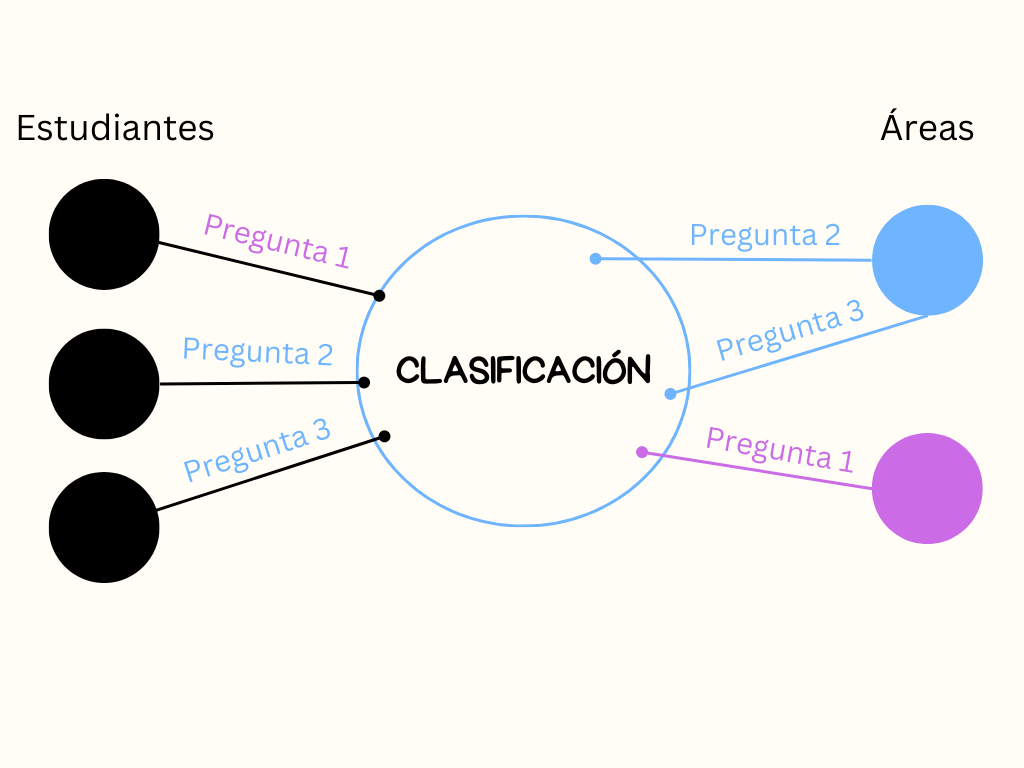
\includegraphics[width=15cm, height=11.25cm]{clasification.png}
	\caption{Mecanismo de clasificación}
	\label{fig:clasification}
\end{figure}

\begin{figure}[h]
	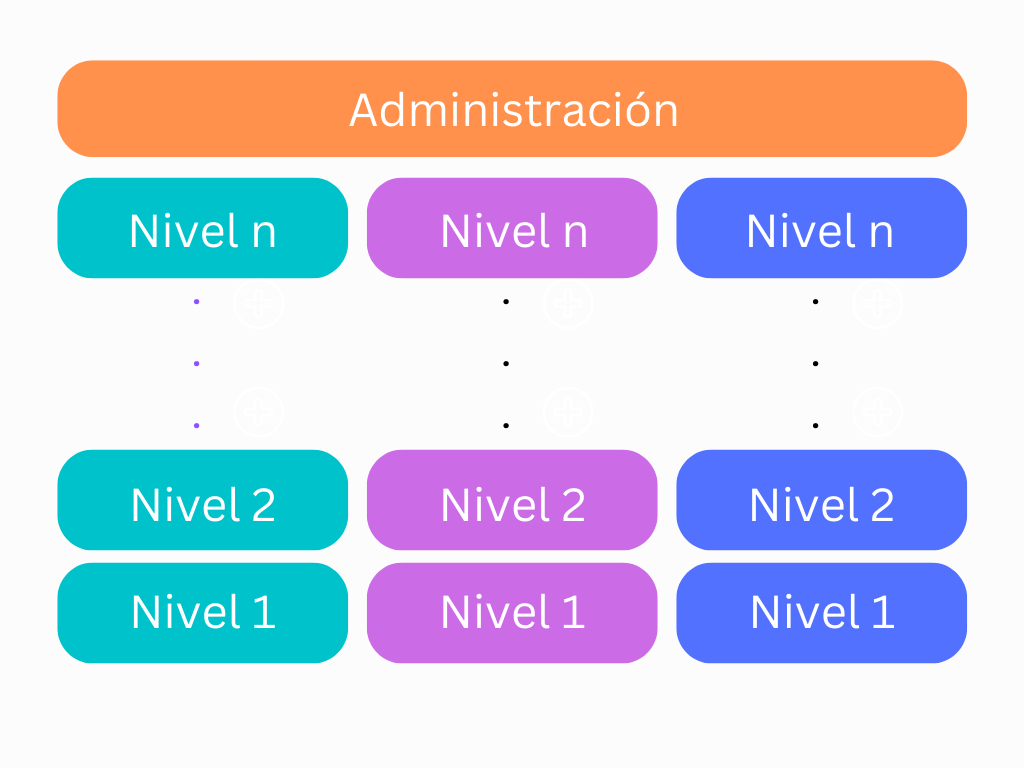
\includegraphics[width=15cm, height=11.25cm]{hierarchy.png}
	\caption{Jerarquía}
	\label{fig:hierarchy}
\end{figure}


\begin{figure}[h]
	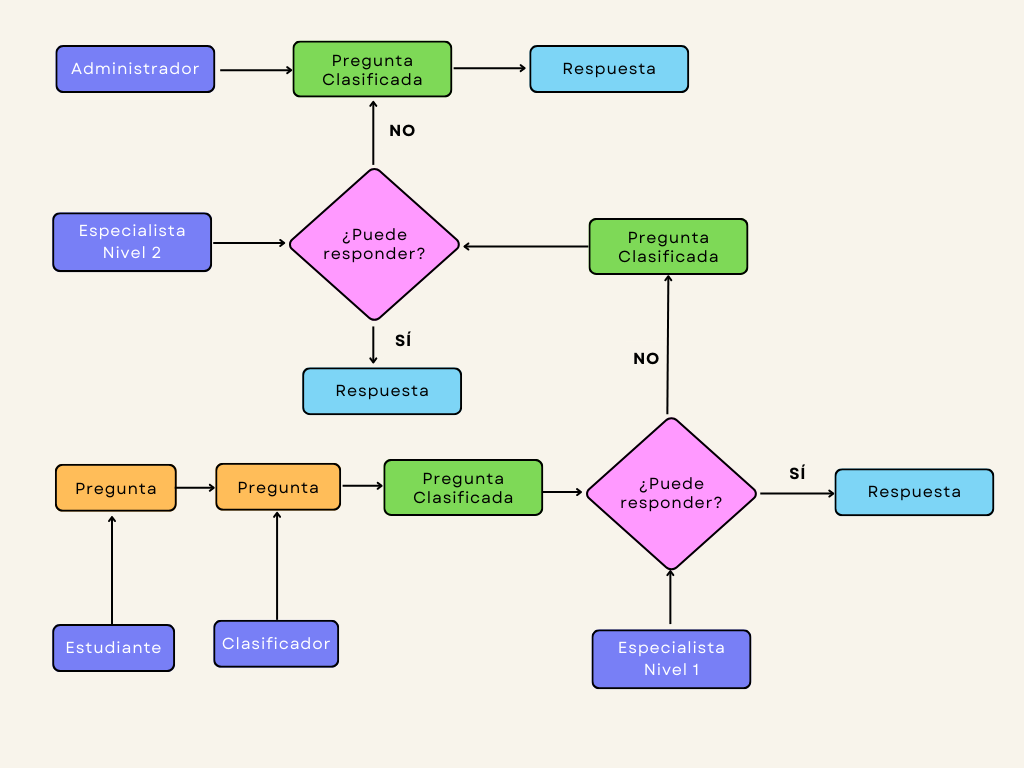
\includegraphics[width=15cm, height=11.25cm]{thesis_diagram.png}
	\caption{Propuesta del sistema}
	\label{fig:myprop}
\end{figure}


